\documentclass{standalone}

\usepackage{tikz,tikz-3dplot,pgfplots,xcolor}
\usetikzlibrary{arrows.meta,calc}

%\pgfplotsset{compat=1.18} 
\definecolor{gray0}{rgb}{0.98,0.98,0.98}
\definecolor{gray1}{rgb}{0.8,0.8,0.8}
\definecolor{gray2}{rgb}{0.7,0.7,0.7}

\begin{document}

  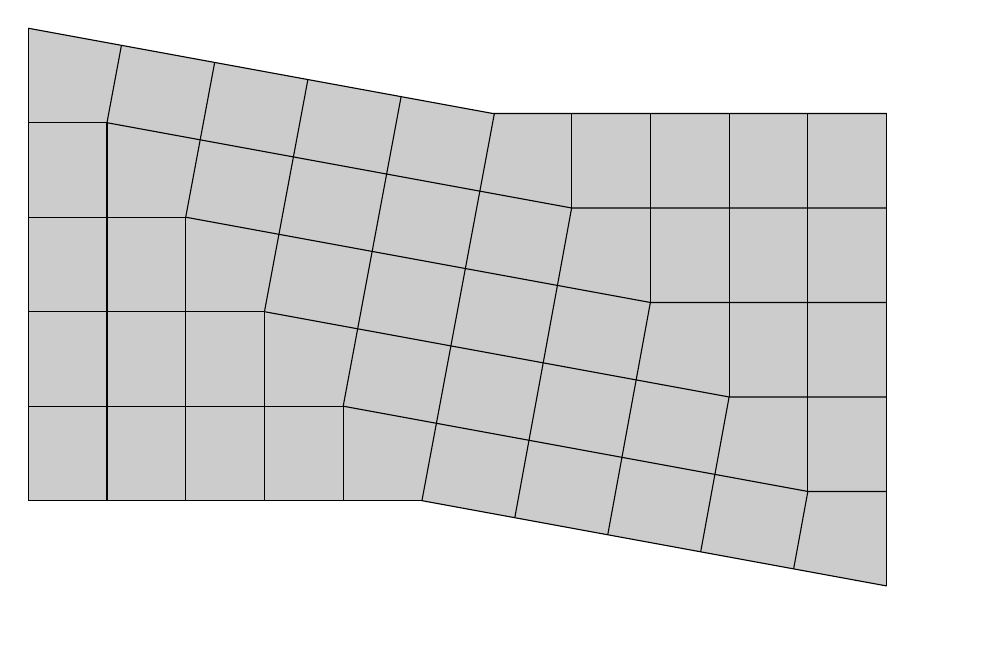
\begin{tikzpicture}[>=Latex]
    \path (0,-1.5) rectangle (12,6);
    \path[fill=gray1] (0,0) coordinate(a) --++ (5,0) coordinate(b) --++ (-10.4:6) coordinate(c) --++ (0,6) coordinate(d) --++ (-5,0) coordinate(e) --++(169.6:6) coordinate(f) --cycle;

    \foreach \x in {0,...,5}{
      \draw (\x,0) -- (\x,6-1.2*\x) ;
      \draw (0,1.2*\x) -- (5-\x,1.2*\x); 
      \draw (5-\x,1.2*\x) --++ (79.4:5-\x); 
      \draw (\x,6-1.2*\x) --++ (-10.4:6) coordinate (cc) --+ (5-\x,0);
      \draw (cc) --+ (0,1.2*\x);
    }
    \foreach \x in {1,...,5}{
      \path (\x,6-1.2*\x) --++ (-10.4:6) coordinate (cc);
      \draw (cc) --+ (259.6:5-\x);
    }

  \end{tikzpicture}
\end{document}